\chapter{Проектирование}
\label{cha:ch_1}

\subsection{Класс совместимых приложений}
Описанный в данной работе набор ассетов Automated Test Framework (ATF) предназначен для автоматизации действий с целью функционального тестирования. Его можно интегрировать c любым  \textit{Unity}-проектом, система ввода которого построена вокруг класса из стандартной библиотеки \textit{Unity} по взаимодействию с вводом Input. Под это описание подходит большая часть \textit{Unity}-приложений и в этом выражена универсальность предложенного решения. Ранее среди свободных для использования ассетов не было представлено решений для автоматизации ни success-тестов, ни тестирования главного потока сценария использования (use-case), ни других подходов для функционального тестирования приложений, кроме как через механизмы стандартного пакета unit-тестирования \textit{Unity}. Однако как бы ни был хорош подход использования инструментария unit-тестирования, для того чтобы покрыть все возможные сценарии действий внутри проекта, пришлось бы либо писать свой модуль тестов под каждый из аспектов, либо же на его основе реализовывать сложную универсальную систему.

\subsection{Определение теоретической базы}
\begin{figure}[H]
	\centering
	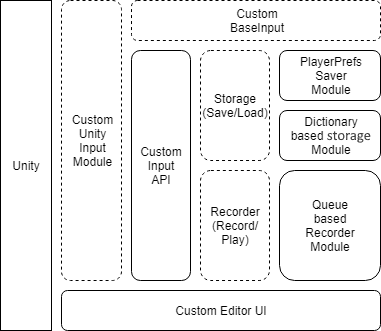
\includegraphics[width=\linewidth]{platform.png}
	\caption{Диаграмма платформы решения}
	\label{platform}
\end{figure}

На этапе проектирования была составлена диаграмма платформы (см. рис. \ref{platform}), каждый блок которой -- это изолированная группа методов API, решающая свои задачи: 
\begin{itemize}
	\item \textit{Unity} -- непосредственно сам игровой движок;
	\item \textit{Custom Unity Input Module} -- абстракция, объединяющая управление вводом;
	\item \textit{Custom Input API} -- собственно API, который вызывает нативные методы по запросу ввода;
	\item \textit{Custom BaseInput} --  сущность, которяа является реализацией объекта обработки потока данных через мост (Bridge), объединяя статичные методы по перехвату/симуляции ввода и обернутые события (Events);
	\item \textit{Storage} --  абстракция, отвечающая за функционал хранения и манипуляции записанных действий;
	\item \textit{Recorder} -- абстракция, отвечающая за запись действий;
	\item \textit{Custom Editor UI} -- система пользовательских окон для управления всеми процессами;
	\item \textit{PlayerPrefs Save/Load Module} -- система реализации абстракции модуля по сохранению/загрузке записанных действий на базе стандартного класса PlayerPrefs;
	\item \textit{Dictionary based Module} -- реализация абстракции хранилища записанных действий, основанная на структуре данных ``Словарь'';
	\item \textit{Queue based Recorder Module} -- реализация абстракции, отвечающей за запись действий, основанная на структуре данных ``Очередь''.
\end{itemize}

Для выполнения поставленных задач было разработано решение, являющееся, по своей сути, модифицированным адаптером, который перехватывает и симулирует ввод. Для его эффективной реализации стало органичным использовать несколько архитектурных паттернов:
\begin{itemize}
	\item
	\textit{Interceptor} -- шаблон для перехвата и подмены входных данных с периферийных устройств \cite{interceptor};
	\item
	\textit{Broker} -- шаблон для интеграции и взаимодействия с встроенной системой управления входными данными \textit{Unity} \cite{broker};
	\item
	\textit{PAC (Presentation–abstraction–control)} -- шаблон для организации взаимодействия зависимых систем \cite{pac}.
\end{itemize}

Для подмены стандартного класса Input был создан перехватчик ATFInput (см. рис. \ref{atfInput}), который наследуется от стандартного класса BaseInput для использования встроенной пользовательской системы управления вводом. ATF -- это сокращение от английского Automated Test Framework, которое переводиться как: фреймворк автоматизированного тестирования. Так как класс Input содержит в себе только статичные методы, декорация их для перехвата внутри ATFInput позволила совместить и классический перехват ввода и облегчить в дальнейшем перехват событий ввода. Иначе говоря, было проведено совмещение перехватчика для класса Input и класса BaseInput  для взаимодействия с событиями ввода внутри \textit{Unity}. 

\begin{figure}[H]
	\centering
	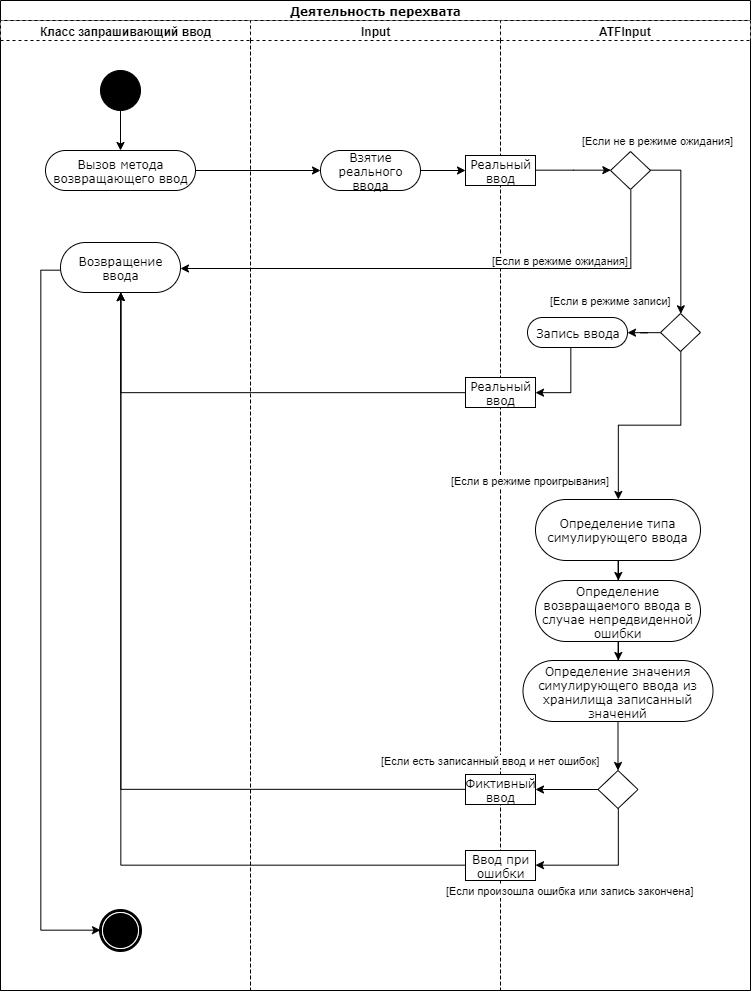
\includegraphics[width=\linewidth]{atfInput.png}
	\caption{Диаграмма деятельности ATFInput}
	\label{atfInput}
\end{figure}


Для интерпретации (проигрывания) первоначально использовался паттерн Interpreter с терминалами ожидания внутри Coroutine. Однако после попытки тестовой реализации данного шаблона был произведен отказ от этого шаблона в пользу метода записи, основанного на структуре данных ``Очередь'', так как для правильной работы терминалов ожидания необходимо было просчитывать заранее действия пользователя, что затруднительно.